% BACKGROUND & RELATED WORK
%
% !TEX root = ../thesis-main.tex
%
\chapter{Background and related work}
\label{chap:background}

%\cleanchapterquote{You can’t do better design with a computer, but you can speed up your work enormously.}{Wim Crouwel}{(Graphic designer and typographer)}




\section{Computer-Assisted Pronunciation Tutoring} %TODO Teaching,Training?

In the field of second-language education, pronunciation has traditionally been given less attention than other areas such as grammar or vocabulary \parencite{Derwing2005}. One reason for this may be that pronunciation is best taught through one-on-one instruction, which is not often possible in the traditional classroom setting. Hence the attraction of Computer-Assisted Pronunciation Training (CAPT) systems, which have the potential to automatically provide highly individualized analysis of learner errors, and feedback on how to correct them and achieve more intelligible and native-like pronunciation in the target language \parencite{witt2012}. 

	\subsection{Pronunciation in foreign language education}


	\subsection{Computer-based and intelligent tutoring systems} 
	%TODO is this section necessary?
	
	\subsection{Survey of existing CAPT systems}
	
	

\section{Towards CAPT for French learners of German}
\label{sec:CAPT4FG}

	\subsection{Phonetic and phonological comparison}
	\label{sec:CAPT4FG:comparison}
		\subsubsection{Segments}
		\subsubsection{Prosody}
		\subsubsection{Other factors}
		
	\subsection{Targeting lexical stress errors}
	\label{sec:CAPT4FG:targeting}
	Learners of a foreign language typically make a wide variety of pronunciation errors, at both the segmental level (e.g. errors in producing certain individual phones of the target language) and the prosodic level (e.g. errors in the speaker's intonation contour or the duration of certain syllables or words). As it is not possible to address all of these in an automated system, one of the first aims of this work is to identify a single type of error which is well suited to being addressed via a CAPT system targeting French L1 learners of German as the L2. 
	
	To guide this selection, we propose a set of three criteria that such an error must meet. First, the error must be produced with a some degree of frequency by French L1 speakers in their production of L2 German, as it would be a misuse of resources to design a system which addresses an error that is seldom made by learners. Secondly, the given error must have a significant impact on the perceived intelligibility of the learner's speech; as the ultimate goal of the system is to help learners communicate more effectively in the L2, an error which is commonly made but nevertheless does not impede understanding of the learner's L2 speech, and thus does not hinder communication in the L2, is not an ideal target. Finally, in order for the CAPT system to provide any meaningful diagnosis of and feedback on the error, it must lend itself to reasonably accurate and reliable  detection through automatic processing. 
	
		%\begin{center}
		\begin{figure}[htb]
			\centering
			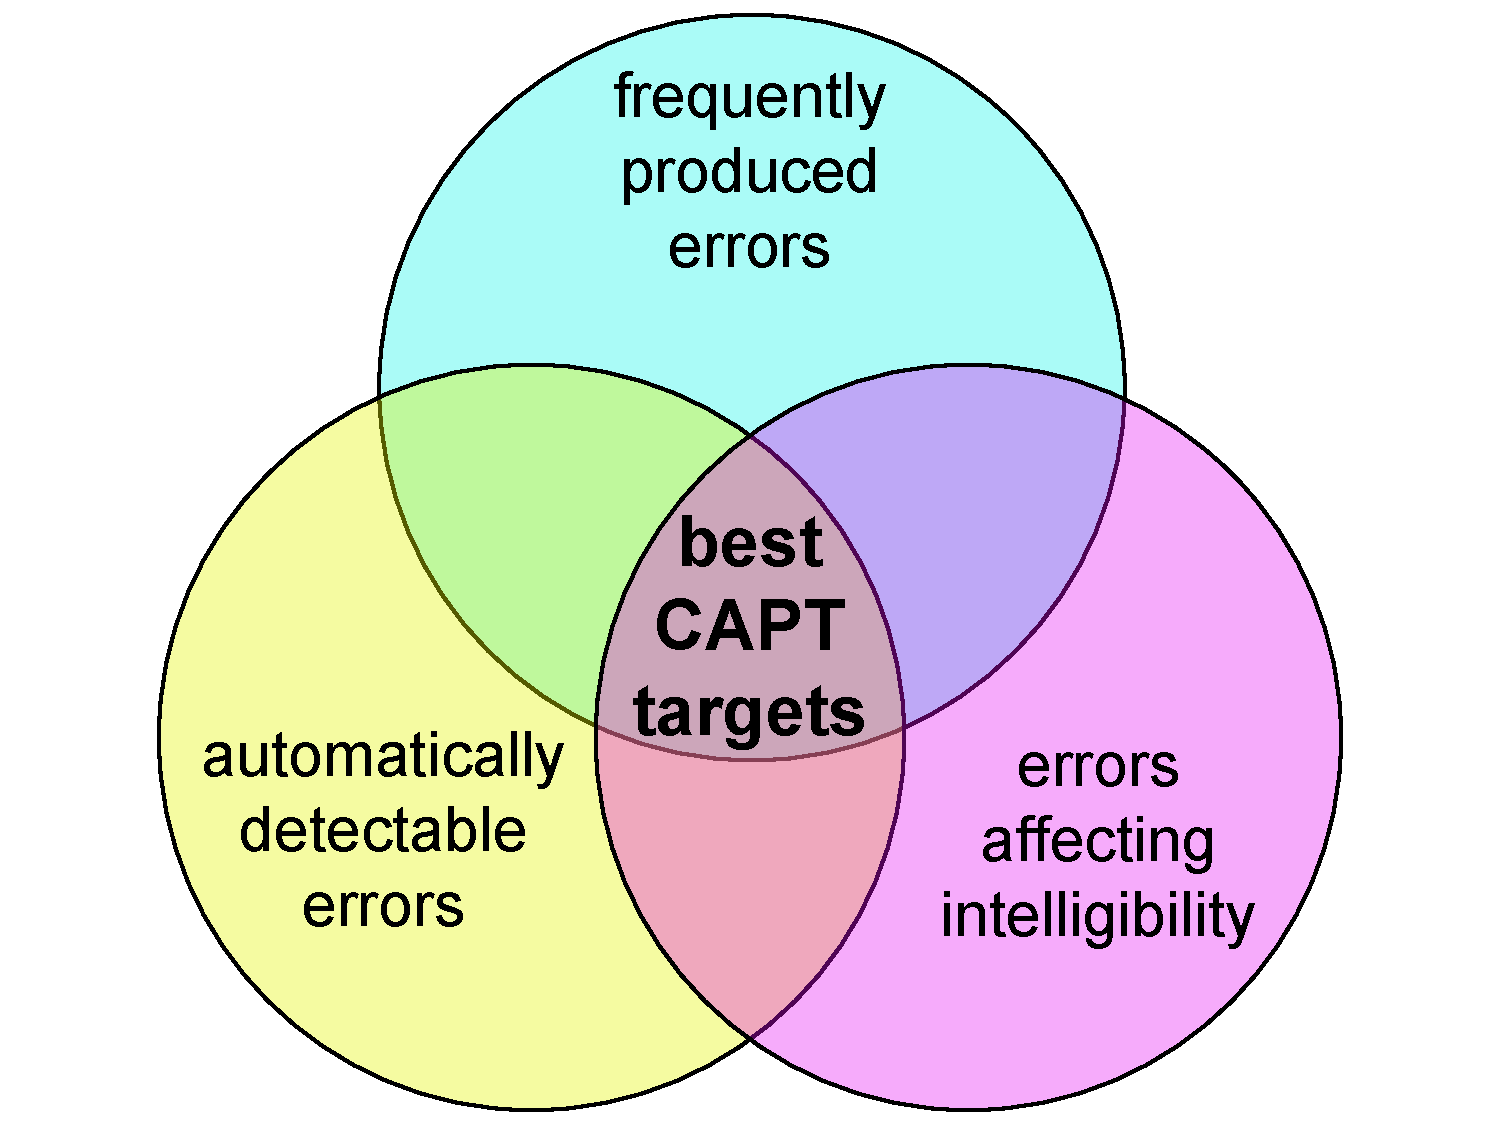
\includegraphics[width=.7\textwidth]{../img/error-venn}
			\caption{Criteria for selecting errors to target in a CAPT system.}
			\label{fig:errors}
		\end{figure}
		%\end{center}
	
	 As illustrated in \ref{fig:errors}, the best error to target with the CAPT system will fulfill all of these criteria, rather than only one or two of the three. 
	 %TODO take the below out?
	 For example, vowel quality errors (e.g. an L1 French speaker producing a German /\textipa{@}/ as [\textipa{\oe}]) may occur frequently in the L2 speech and may be relatively easy to detect automatically, but may not have a great impact on the intelligibility of the L2 German speech. On the other hand, equally frequent vowel quantity errors (e.g. the L1 French speaker producing a German long /\textipa{e:}/ as [\textipa{e}]) may have a greater impact on intelligibility in some cases, but may be more difficult to reliably identify automatically.
	
	Analysis of the typical and expected errors described in \label{sec:CAPT4FG:comparison} in terms of these criteria reveals that lexical stress errors are a strong candidate for treatment via CAPT, and will therefore be the focus of the prototype CAPT system described in this thesis. The remainder of this section justifies the selection of this type of error by describing how it fulfills the aforementioned criteria as well or better than any other error type.
	

	

		
		\subsubsection{Frequency of production}
		
		\subsubsection{Impact on intelligibility}
		\cite{Warren2009}, \cite{Magen1998}
		
		\subsubsection{Feasibility of automatic detection}
		\cite{ISADEPT, delmonte2011}
		
\section{Summary}